\section{Current observability problems}
    The problem we are trying to tackle can be described by the following situation: 
    Imagine an Erlang application instrumented with OpenTelemetry. Suddenly, the application starts slowing down, and the execution of a function takes 10 seconds. The engineer knows it should take at most 1 second. Between its start and its end, no information about the span appears on the dashboard.
    
    We believe that this is a problem. One would like to know right away if something is wrong with their application. This is where the $\Delta$QSD paradigm and the $\Delta$Q oscilloscope come in handy. \\ 
   Using $\Delta$QSD, we can set a maximum delay ($dMax$) for a task. As soon as the maximum delay is hit, the oscilloscope is notified right away that there is a problem.
   
   \begin{figure}[H]
        \begin{center}
            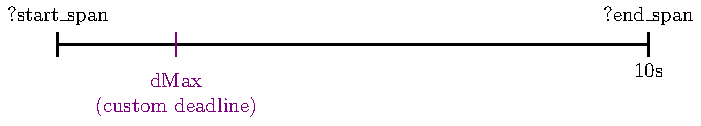
\includegraphics{tikz/start_end_dmax.pdf}
        \end{center}
        \caption{Execution of a long span in OpenTelemetry. Normally, the user will be notified after 10 seconds that the function has ended. The $dMax$ deadline gives an early notification that the span has taken too long.}
        \label{fig:otel_dmax}
    \end{figure} 


    \subsection{Handling of long spans}
        OpenTelemetry presents a bigger problem, what happens when there are long-running spans? Even worse, what happens when spans are not actually terminated?
        
        An article has already tackled this problem \cite{otel-l}. In the article it is stated that OpenTelemetry limits the length of its spans, moreover, those who are not terminated are lost and not exported. \\ 
        In addition, it is said that if the span is the parent/root span, its effect could trickle down to child spans. We can quickly see how this can become problematic, all the information about an execution of your task is lost. A span can apparently not be terminated for trivial reasons: refreshing a tab, network failures, crashes. The author states that there are a few solutions that can be implemented: having shorter spans, carrying data in child spans, saving spans in a log to track spans which were not ended to manually set an end time. The solutions have been implemented by the Embrace (commercial) monitoring tool \cite{embr}, but it is apparently the only tool out of the ecosystem of monitoring tools.

     We believe that the adapter we provide can be a great start to improve observability requirements surrounding OpenTelemetry. Data about spans will always be carried to the oscilloscope, whether the span is long or non-terminated. This is further developed in Chapters 3 \& 5.
